\section{Results}

% 1 page
%Renan: Results-Intro
%TODO Gabriel: Results-Calibration
%Estevão: Results-Mecanica
%Renan: Results-Control

% Intro

Simulations and experimental tests were performed to verify the proposed
concepts. The following results were divided according to the EMMA system's
elements introduced in Sec.~\ref{solution}. 


\subsection{Robotic manipulator analysis}\label{sec::man_analysis}

As stated in Subsec.~\ref{manipulator}, simulations for the robotic
manipulator were implemented with OpenRave, and consist of the following steps:
blade's surface discretization; coating strategy; base position computation;
kinematics, dynamics and manipulability.

The blade's surface discretization is an uniform sampling to
determine where to the coating directions should be. However, sampling the
actual geometric surface can lead to unwanted results due to possible
concavities. A simpler approach is to take the bounding box of the blade and
sample its surface uniformly. Once the
surface of the box is sampled, the intersection of the blade and a ray
originating from each point going inward is taken. The normal of the blade's
surface from each of these intersection points is taken to be the coating
direction. As an uniform sampling of the box does not mean an uniform sampling
of the blade, the box is oversampled and a 50~mm filter is applied, by a multidimensional search key with k-d tree.
The samples are translated 230~mm in respect with their normal vectors,
collision checks with the environment are made, and the feasible samples are
named \textit{coating samples}. Fig.~\ref{fig:discretization} shows the
\textit{coating samples}. 

Base position computation is to uniformly sampling the turbine's
confined space and calculate the required robotic manipulator's base positions
to process all the \textit{coating samples} in angle and distance tolerances.
It is a brute force search: for each position, inverse kinematics (IKFast) are
computed to determine the robotic manipulator's joint parameters that provide
the desired positions and orientations of the end-effector.
Fig.~\ref{fig:coating} shows examples of the algorithm, where black dots are
coated points and blue dots are coated points with angle tolerance. At the end
of the algorithm, the \textit{reachable samples} relate coating samples with base
positions, thus it is possible to create a coating strategy and to select the
simplest base positions. The result is the minimum required positions for the
robotic manipulator's base.

\begin{figure}
	\centering
	\subfigure[Blade
	discretization.]{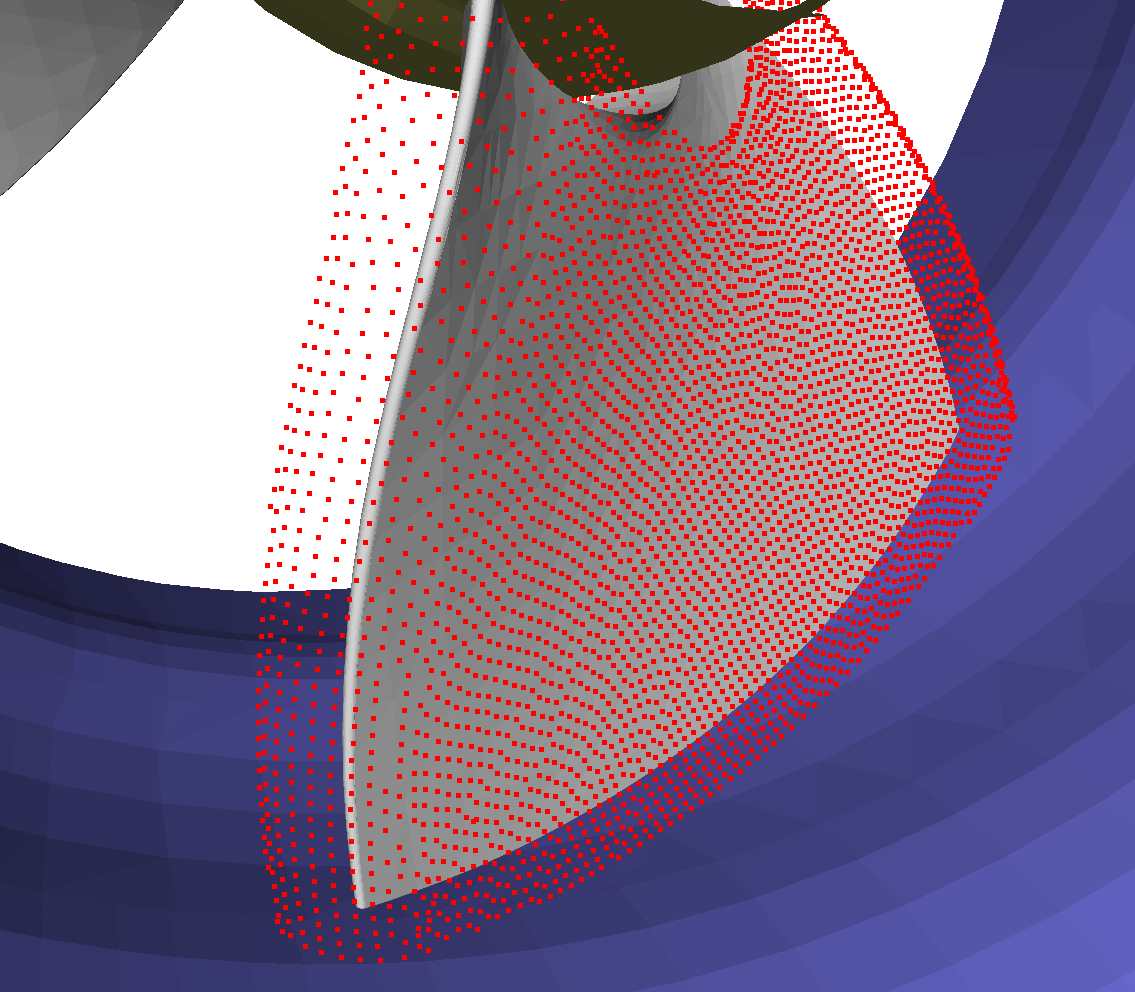
\includegraphics[width=0.46\columnwidth]{figs/results/blade_grid1.png}\label{fig:discretization}}
	\quad
	\subfigure[Coating
	example.]{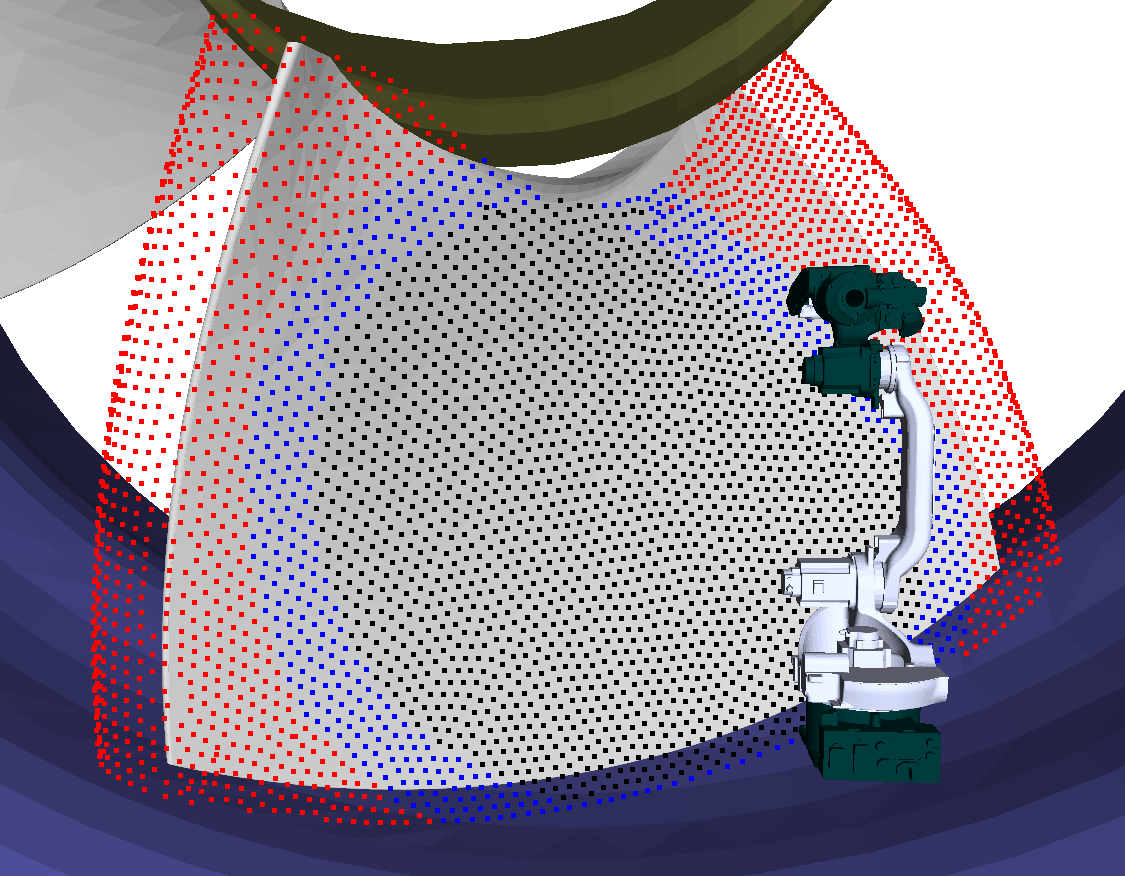
\includegraphics[width=0.47\columnwidth]{figs/results/mh12_coating2.png}\label{fig:coating}}
\end{figure}

\begin{comment}
\begin{algorithm}
\caption{Coating strategy}
\label{alg:strategy}
\begin{algorithmic}[1]
\ForAll{Base positions} 
		\ForAll{\textit{Coating samples}}
			\State Joints = IKFast(sample)
			\If{not Joints} 
				\State Joints = IKFast(sample,tol)
			\EndIf
			\If{Joints} 
				\State $\textrm{Reachable}[\textrm{pos}] += [\textrm{sample}]$
				\label{algvar:reachable}
			\EndIf
		\EndFor
\EndFor
\end{algorithmic}
\end{algorithm}
\end{comment}

The kinematic approach described above is not enough to ensure that the robot
will reach the \textit{coating samples}. Maximum accelerations, decelerations,
torques, and jacobian singularities should be investigated and compared to the robotic
manipulator's specifications. The Newton-Euler method
\cite{sciavicco2000differential} was adopted for torque computation: $\tau =
M(q)\alpha + C(q,\omega)\omega + G(q)$, where $\tau$ is the joints' torques,
$M$ is the matrix of links' masses and moments of inertia, $\alpha$ is the
joints' accelerations, $q$ is the joints' angles, $\omega$ is the joints'
velocities, $C$ is the Coriolis matrix, and $G$ is the gravity vector.

In the dynamic approach, $M$ was estimated by the robotic manipulator's CAD
model. The angular accelerations are derived by differential kinematics:
$\alpha=J^+(a-\omega^TH\omega)$, where $H$ is the Hessian matrix
\cite{hourtash2005kinematic}, $a=\ddot{X}$ is the linear accelerations, and $J$
is the Jacobian matrix. Therefore, torques can be analytically estimated with
the inverse dynamics in OpenRave. Comparing estimated torques with the technical
specifications, dynamic simulations's results showed that the robotic
manipulator should be placed at, at least, 1400~mm distance from the blade's
surface plane. Placing the robot nearer would enhance the robotic manipulator's
workspace, but it would increase also the torques. The Fig.~\ref{fig:torques}
is an example of the robotic manipulator in a close range, 900~mm distance from the
blade. It shows joints' torques for blades's \textit{coating samples} in a color
gradient way, where red dots represents small magnitudes and blue dots are large magnitudes. 

\begin{figure}
	\centering
	\includegraphics[width=.5\columnwidth]{figs/results/manipulability_colorgradient.png}
    \caption{Robotic manipulator joints' torques in color gradient.}
    \label{fig:torques}
\end{figure}

\subsection{Base analysis}

The FEA of the base verifies the Von Mises stress and the displacements
along the structure's slender members. The stress analysis determines the
integrity of the base due to the maximum loads of the robotic manipulator. The
displacements determine if the structure provides a rigid base for the robotic
manipulator. According to the hard coating requirements, displacements of the
order of millimeters are not allowable in the elastic region of the
material. 

The FEA solver was the Nastran In-CAD$^{\mbox{\small\textregistered}}$ with
SolidWorks$^{\mbox{\small\textregistered}}$. Model's elements are 1-D 
\textit{bar line elements} with a global mesh's size of 25~mm. The material's
properties are: density 2700~$kg/m^3$; Young modulus 70~GPa; Poisson's ratio
0.34; and Yield strength 200~MPa. Boundary conditions are three translational
constraints for the anchors and a vertical constraint to the feet. The
rotational joint is modeled as a rigid connector between the rails, such as the
robot's base with respect to the second rail. The robotic manipulator's maximum
dynamic forces and moments are applied, as static loads, to the point that
represents the origin of the robot's base.

The maximum Von Mises stress was 4.16~MPa (Fig.~\ref{fig:von_mises}), which
gives a factor of safety of 34.6. It was found for a particular case where the robotic manipulator is in
the secondary rail, 800~mm from the rotational joint. The displacement of the
structure causes a maximum translation of 0.47~mm and a angular deflection of
$0.0149^{\circ}$ in respect to robotic manipulator base's coordinate system. 

The field tests conducted in the draft tube for the magnetic fixtures, at
different equipment's orientations and places, confirmed the manufacturer's
payload capacity. As the maximum tractive reaction force obtained in FEA
simulations was 956~kgf, it was chosen a magnetic fixture with 1200~kgf
capacity.

\begin{figure}
	\centering
	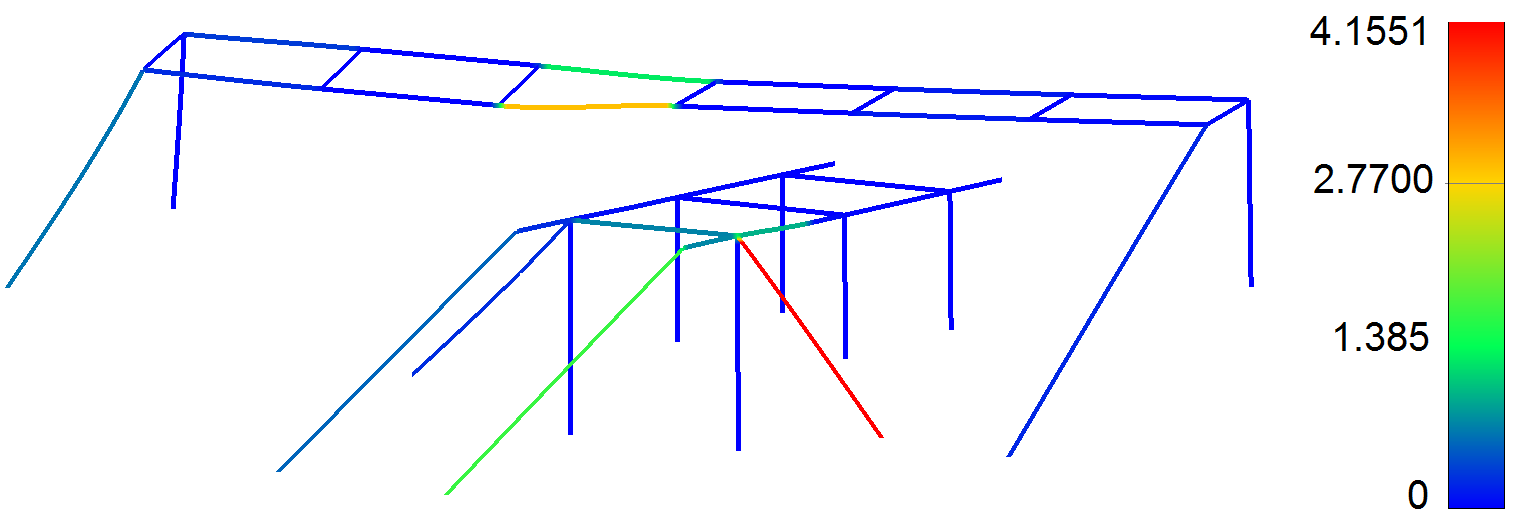
\includegraphics[width=.95\columnwidth]{figs/mecanica/von_mises.png}
    \caption{Von Mises's stress result.}
    \label{fig:von_mises}
\end{figure}

\subsection{Calibration analysis}

Field tests are very complex due to the logistics and the availability of a dry
hydropower turbine, thus simulated data were analyzed, which can be consistent
and can represent effectively the actual operation scenario. In calibration
analysis, turbine's environment and the robotic manipulator were simulated with
the toolbox Blensor \cite{Gschwandtner11b}. The blade's model, however, was
acquired in a field test by a 3D laser scanner for a better representantion of
the actual hidraulic profile.

The laser sensor was modeled following manufacturer's technical
specifications, and different scenes were generated for several sensor's
positions. The algorithm is able to localize the blade in respect to the
sensor's coordinate system, even in occlusion by the presence of the robotic
manipulator. In Fig.~\ref{fig:calibration}, the left yellow blade is the
reference model, the red blade is the object to be found, and green lines
represent the matching features between the model and the scene.

\begin{figure}
	\centering
	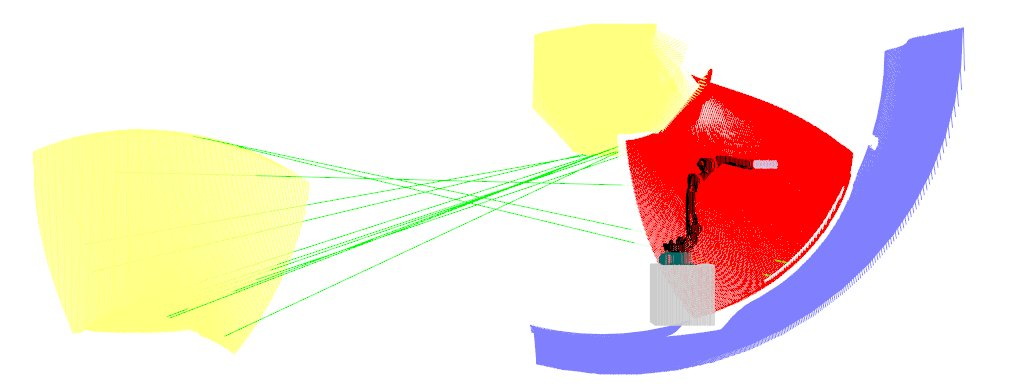
\includegraphics[width=.95\columnwidth]{figs/results/sim_mh12_sp}
    \caption{Robotic manipulator joints' torques in color gradient.}
    \label{fig:calibration}
\end{figure}